\newpage % Rozdziały zaczynamy od nowej strony.
\section{\label{embeddings}Embeddingi}

\subsection{Czym jest embedding słów}
% zrodło https://towardsdatascience.com/neural-network-embeddings-explained-4d028e6f0526
% zrodlo 2 https://www.tensorflow.org/tutorials/text/word_embeddings
% -----  https://developers.google.com/machine-learning/crash-course/embeddings/video-lecture

% ---- https://en.wikipedia.org/wiki/Word_embedding

% https://pathmind.com/wiki/glossary#cosine

% https://machinelearningmastery.com/what-are-word-embeddings/


Embedding słów jest to zbiorcza nazwa na techniki i narzędzia wykorzystane w ramach przetwarzania języka naturalnego pozwalające na dokonanie mapowania słów, ze zbioru znanych pojęć, na wektor liczb rzeczywistych. Z matematycznego punktu widzenia sprowadza się to do transformacji z dyskretnej przestrzeni o wielu wymiarach do ciągłej przestrzeni ze znacznie mniejszą liczbą wymiarów. \cite{Emb_def}
% zrodlo ----> https://en.wikipedia.org/wiki/Word_embedding

%Word embedding is the collective name for a set of language modeling and feature learning techniques in natural language processing (NLP) where words or phrases from the vocabulary are mapped to vectors of real numbers. Conceptually it involves a mathematical embedding from a space with many dimensions per word to a continuous vector space with a much lower dimension.


Takie podejście powoduje, że możliwe jest badanie podobieństwa słów wykorzystując cosinusowe podobieństwo. Jeśli dwa słowa mają podobne znaczenia lub wykorzystywane są w podobnym kontekście  wartość podobieństwa będzie bliższa jednemu. Jeśli słowa rzadko ze sobą występują wartość podobieństwa będzie bliższa zeru.  \cite{cooos_def}

%todo: można dodać wzór na liczenie...



%zrodlo -> https://www.tensorflow.org/tutorials/text/word_embeddings

%Word embeddings give us a way to use an efficient, dense representation in which similar words have a similar encodin



\subsection{Wykorzystane embeddingi}
W ramach pracy są wykorzystywane trzy rodzaje embeddingów, każdy z nich różni się długością wektora i sposobem jego uzyskania. Wykorzystane w pracy embeddingi to:
\begin{itemize}
    % \item Word2vec
    \item Glove
    \item FastText
    \item ELMo
\end{itemize}



\subsubsection{Word2vec}
Metoda ta nie została wykorzystana w pracy, jednak jest ona kluczowy do zrzumienia podstaw działania i tworzenia ebeddingów dlatego zostanie omówiony w tej sekcji. Występuje w dwóch odmianach:

\begin{itemize}
    \item CBOW
    \item Skip grams
\end{itemize}



Tworzenie embeddingu w oparciu o model typu CBOW polega na trenowaniu prostej sieci neuronowej. Sieć ta składa się z warstwy wejściowej, jednej warstwy ukrytej (warstwy gęstej) oraz warstwy wyjściowej. Trening modelu polega na podawaniu na wejście słów mieszczących się w ramach pewnego założonego okna, przewidując słowo będące w środku tego okna. Jako okno rozumie się tutaj stałą liczbę słów przed i po aktualnie przewidywanym słowem. Słowa, by mogły być przewidywane przez model, są wcześniej konwertowane do przestrzeni wektorowej poprzez wykorzystanie one-hot encodingu. Proces uczenia polega na systematycznym przesuwaniu okna o jedno słowo i trenowanie wag w warstwie ukrytej. Po zakończonym procesie uczenia należy usunąć ostatnią warstwę wyjściową, a wagi z warstwy ukrytej,wykorzystać do uzyskanie embeddingu słów.\cite{Mikolov2013}

Odmiana ‘skip grams’ jest analogiczna do metody CBOW, tylko zamiast przewidywania jednego słowa w kontekście jego otoczenia, przewidywane jest otoczenie w kontekście słowa.


\subsubsection{Glove}
% https://nlp.stanford.edu/pubs/glove.pdf

Metoda opiera na wykorzystaniu globalnych statystyk współwystępowania słów\cite[]{Pennington2014}, zamiast wykorzystywania tylko informacji o lokalnym kontekście, jak jest to czynione w ramach metody word2vec. Współwystępowanie słów jest zliczane w ramach stałego okna, w ramach które wchodzi skad 10 słów z lewej i z prawej strony.

Trenowanie modelu polega na wyznaczeniu takich embeddingów słów by ich iloczyn skalarny był równy logarytmowi prawdopodobieństwa współwystępowania tych słów w korpusie. Jest to opisane poniższym wzorem:

%todo
% //wstwaić wzór i opisać jego elementy
% \colorbox{yellow}{todo:}\\

$$w_i^T \tilde{w_k}   = log(P_{ik}) = log(X_{ik}) - log(X_i)$$
gdzie: \\
$w_i$ - embedding słowa \textbf{i} \\
$w_k$ - embedding słowa  \textbf{k} \\
$X_{ik}$ - liczba razy, gdy słowo \textbf{k} występuje w kontekście słowa \textbf{i} \\
$P_{ik} = P(k|i) = X_{ik}/X_i $- prawdopodobieństwo, że słowo \textbf{k} wystąpi w kontekście słowa \textbf{i}\\
$X_{i} = \sum_{k} X_{ik} $ - liczba razy, gdy jakiekolwiek słowo pojawiło się w kontekście słowa  \textbf{i} \\



% \begin{figure}[!h]
%     \label{fig:wzor}
%     \centering 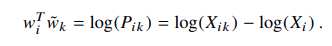
\includegraphics[width=0.5\linewidth]{Selection_016.png}
%     \caption{Wzór: //todo: do przeniesiania dolatexa}
% \end{figure}

\subsubsection{FastText}

Embedding FastText został stworzony w ramach badań prowadzonych przez firmę Facebook\cite{Bojanowski2016}. Jest on wariacją metody word2vec, która rozważa zdanie na jeszcze niższym poziomie. Metoda ta rozbija słowa na jeszcze mniejsze fragmenty, tzw. n-gramy. Dla przykładu, angielskie słowo ‘where’ (dla okna o wielkości n=3) jest rozbijane na następujące części: <wh, whe, her, ere, re>. Badacze dodali także specjalne symbole ‘<’ oraz ‘>’ pozwalające poprawnie identyfikować przedrostki i przyrostki. Także by zachować informację o pełnej formie słowa, słowo to jest także dodane do zbioru n-gramów.

Tak uzyskana interpretacja słowa jest konwertowana do postaci numerycznego wektora. Polega to na dodawaniu wektorów kolejnych elementów zbioru n-gramów do jednego długiego wektora. Tak uzyskane wektory poszczególnych słów są podawane analogicznie jak w przypadku tradycyjnego word2vec na wejścia płaskiej sieci neuronowej pozwalając finalnie wyznaczyć embeddingi słów.

% https://arxiv.org/pdf/1607.04606.pdf
% Enriching Word Vectors with Subword Information

\subsubsection{ELMo}

Ta metoda tworzenia embeddingów nie korzysta już z bezpośrednio z podwalin stworzonych przez metodę word2vec. Zamiast tego do wychwytywania kontekstu słowa, niezbędnego do stworzenia poprawnych embeddingów, wykorzystuje warstwy LSTM \cite{Gardner2017AllenNLP}. Warstwa ta dzięki swojej budowie pozwala na efektywne zapamiętywanie istotnych informacji, z punktu widzenia zagadnienia klasyfikacji, pojawiających się wcześniej w ramach sekwencji danych wejściowych. Więcej infrmacji na temat sieci LSTM zawartych jest w rozdziale \ref{lstm_subsection}.
%todo
% //wiecej szczeŋółów rozdział o wartwaych  ->odnośnik



Przetwarzanie zdania wejściowego odbywa się zgodnie z następującymi krokami:

\begin{itemize}
    \item Zdanie jest dzielone na słowa
    \item Każde słowo, przy wykorzystaniu sieci pomocniczej typu CNN(opierającej się o warswy konwolucyjne), ma przypisywany embedding. Embedding ten jest określany poprzez agregację wektorowej reprezentacji pojedynczych znaków występujących w ramach słowa. Tak uzyskany embedding jest pierwszym elementem finalnego embeddingu (oznaczony jako $E_1$)
    \item Uzyskany wektor jest podawany na wejście pierwszej warstwy Bi-LSTM. Warstwa ta pozwala na analizę zdania zarówno od początku do końca, jak i od końca do początku.
    \item  Stany ukryte z pierwszej warstwy dla każdego słowa są agregowane w jeden wektor i stanowią drugi element finalnego embeddingu (oznaczony jako $E_2$)
    \item Następnie dane o stanie ukrytym pierwszej warstwy są przekazywane na drugą warstwę Bi-LSTM
    \item Stany ukryte z drugiej warstwy dla każdego słowa są agregowane w jeden wektor i stanowią drugi element finalnego embeddingu (oznaczony jako $E_3$)
    \item W ostaniem kroku następuje połącznie uzyskanych fragmentów embeddingów, oznaczonych jako $E_1,E_2, E_3$ w jeden o standardowym wymiarze 1024
\end{itemize}



% //todo: dodać rysunek arch -> bo jest duża fajnych 


%todo: opisać czym są postagi
\subsection{Uwzględnienie POS tagów w ramach embeddingu}


POS tag (Part-of-speach tag) zawiera informacje na temat cech morfosyntatycznych słowa \cite{postags_def}.Najbardziej podstawową kategorią są powszechnie znane części mowy, takie jak czasownik, rzeczownik, przymiotnik. Jednak nie jest to jedyna informacja zawarta w ramach takiego tagu, przechowuje on bowiem także informację o czasie w jakim jest użyty czasownik, w której liczbie jest wykorzystany rzeczownik i wiele innych.

%todo:
% \colorbox{yellow}{todo:}\\
% //todo: można by dorzucić pełną listę, ale to może być problematyczne

% tu jest lista: https://medium.com/@gianpaul.r/tokenization-and-parts-of-speech-pos-tagging-in-pythons-nltk-library-2d30f70af13b

% https://pythonprogramming.net/natural-language-toolkit-nltk-part-speech-tagging/

Aby umieścić informacje na temat części mowy tak by była ona możliwa do interpretacji w ramach embeddingu konieczne jest konwertowanie jej do postaci wektorowej. Ze względu na brak dużego podobieństwa między poszczególnymi częściami mowy zdecydowano się na zakodowanie tej informacji w formie one-hot encoding. Tak utworzony wektor był doklejany do istniejącego już embeddingu uzyskanego innymi metodami tworząc wektor dłuższy o 46 elementów.

%todo:
% //todo: dodać rysunek to obrazujący
% \colorbox{yellow}{todo:}\\



\begin{figure}[!h]
    \label{fig:post_tag}
    \centering 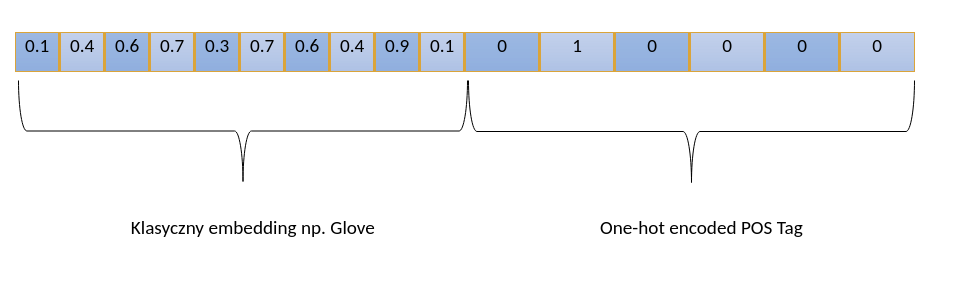
\includegraphics[width=1\linewidth]{post_tag_embedings.png}
    \caption{Przykład embeddingu wraz z zakodowaną informacją o POS tagu}
\end{figure}